%% research goals
\section{One Year Project Horizon}\label{research_plan}
The main objective of this research proposal is to develop novel methods to enable safe and interactive motion planning for autonomous vehicles in urban environments without communication between the agents.

\begin{figure*}[t]
\centering
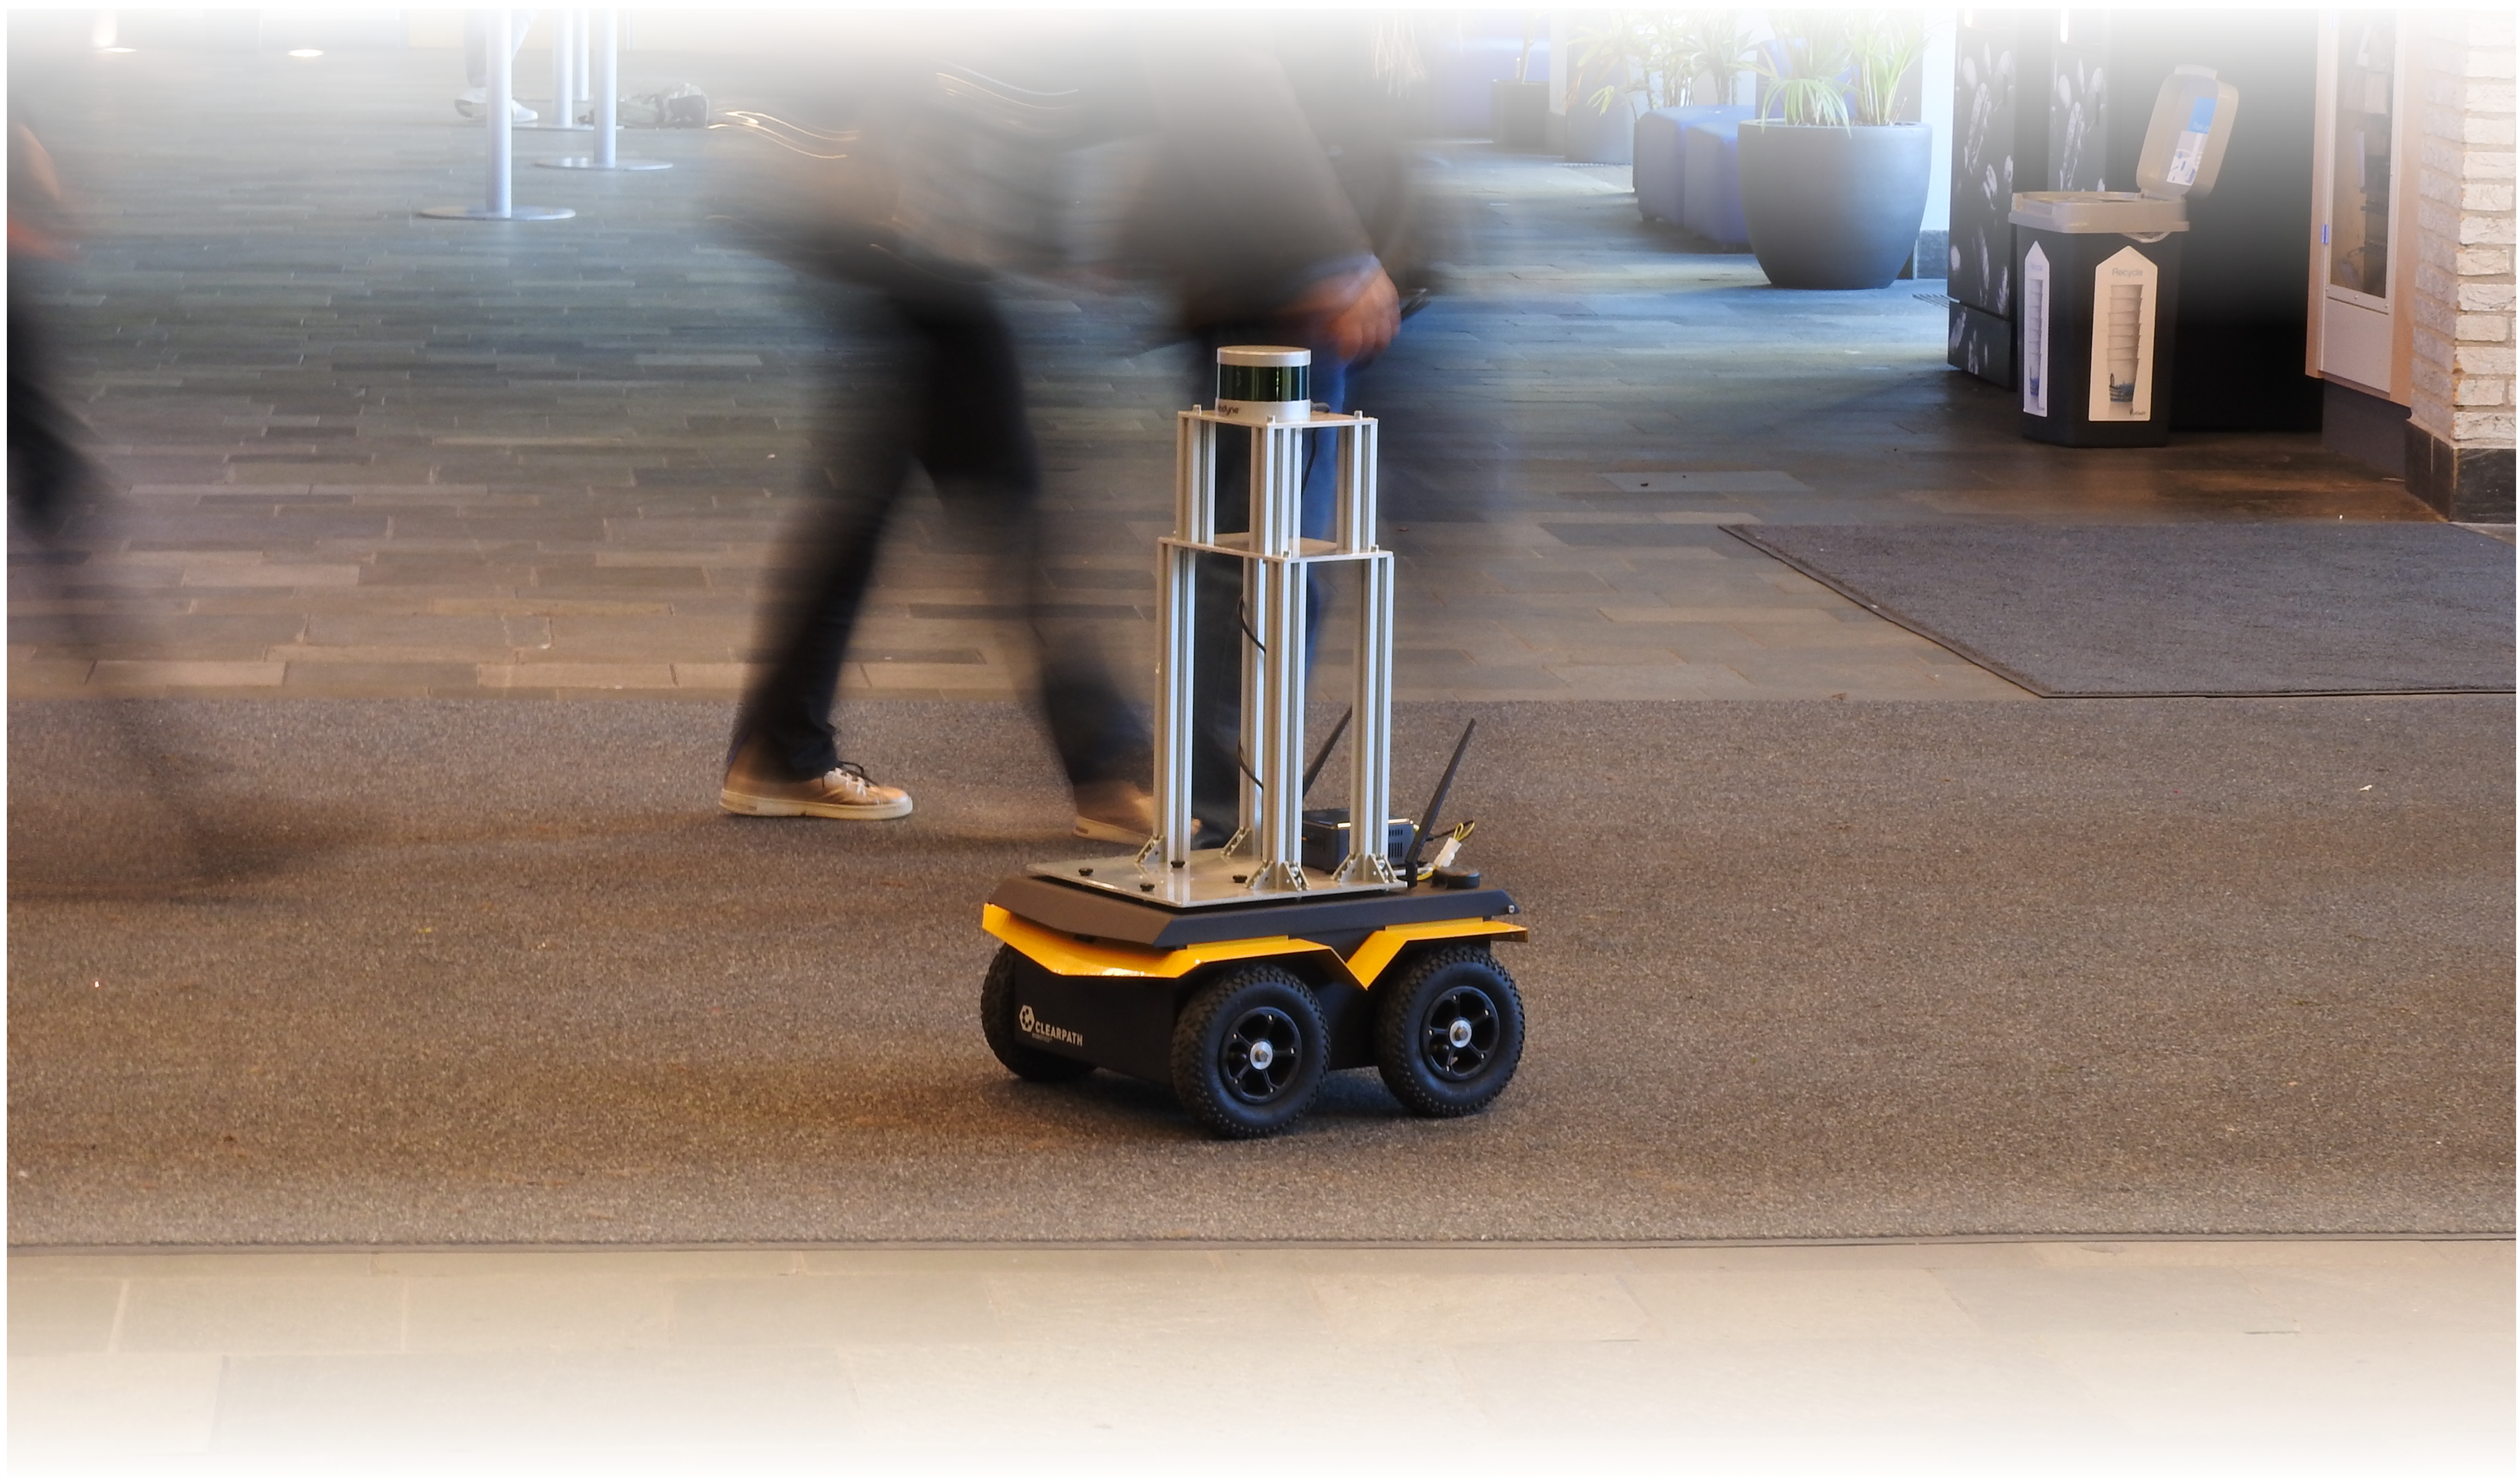
\includegraphics[width=.9\textwidth]{figs/cover.pdf} 
\caption{\emph{S3: experimental results with a pedestrian dummy.} Commanded acceleration, steering wheel angle, and longitudinal velocity of the vehicle.}
\label{fig:experiments}   
\end{figure*} 

\textbf{Month 1-4}The project will beginning with the definition of a set of experiments targeting to record data with scenarios where a mobile robot platform navigates in the same environment as other pedestrians. I will use the Jackal mobile platform presented in Fig. \ref{}.

\textbf{Month 5-8}

\textbf{Month 9-12}

\textbf{Year 3-4}

\section{The strength of the student for achieving the proposal milestones}\label{student}

The proposed research project brings together the fields of robotics, motion planning and machine learning. I have a master in electrical and computers engineering with a major in robotics. Afterwards, I did a 2 years traineeship in the Guidance, Navigation and Control (GNC) section at the European Space Agency (ESA). Here,